\documentclass[../../main.tex]{subfiles}

\graphicspath{{\subfix{../../immagini/}}}

\begin{document}
    Come già accennato, la struttura della rete ricorrente utilizzata negli esperimenti è identica a quella presentata in \cite{ma2020}. Nello specifico, la tipologia di rete ricorrente prende il nome di Gated Recurrent Unit (GRU), che a sua volta è una variante di una più ampia tipologia di RNN chiamata Long Short Term Memory (LSTM).
    
    Intuitivamente, il vantaggio principale delle LSTM (e di conseguenza delle GRU) è la capacità di lavorare su dipendenze a lungo termine, cosa molto difficile nelle RNN, a causa del problema della scomparsa del gradiente. Questa capacità è data dall'aggiunta di un vettore, chiamato cell state $\boldsymbol{C}^{(t)}$, che ad ogni istante di tempo contiene informazioni generate dagli stati precedenti. Ad ogni istante di tempo le informazioni da inserire all'interno del cell state vengono regolate tramite dei `cancelli', o gate.

    In realtà, nelle GRU la funzione del cell state viene inglobata nel vettore $\boldsymbol{n}^{(t)}$ e sono presenti meno gate rispetto ad un LSTM. La figura \ref{fig:strutturaGRU} mostra più nel dettaglio la struttura di una GRU, vengono inoltre riportate di seguito le relative equazioni:

    \begin{flalign}
        \boldsymbol{u}^{(t)} &= \sigma\left(\boldsymbol{W} \boldsymbol{x}^{(t)} + \boldsymbol{U} \boldsymbol{n}^{(t-1)}\right)& \text{gate di aggiornamento,}\\
        \boldsymbol{r}^{(t)} &= \sigma(\boldsymbol{W} \boldsymbol{x}^{(t)} + \boldsymbol{U} \boldsymbol{n}^{(t-1)}) & \text{gate di reset,}\\
        \boldsymbol{\tilde{n}}^{(t)} &= \mathrm{tanh}\left(\boldsymbol{W} \boldsymbol{x}^{(t)} + \boldsymbol{r}^{(t)} \odot \boldsymbol{U} \boldsymbol{n}^{(t-1)}\right) & \text{output intermedio,}\\
        \boldsymbol{n}^{(t)} &= \boldsymbol{u}^{(t)} \odot \boldsymbol{n}^{(t-1)} + (1 - \boldsymbol{u}^{(t)}) \odot \boldsymbol{\tilde{n}}^{(t)} & \text{output finale.}
    \end{flalign}
    Le notazioni qui riportate riprendono quelle del paragrafo \ref{sec:retiRicorrenti}. Inoltre, il simbolo $\odot$ indica l'operazione di prodotto elemento per elemento tra due vettori o matrici.

    Nei nostri esperimenti utilizziamo tre GRU, con uno strato interno $\boldsymbol{n}$ rispettivamente di dimensioni pari a 16,8 e 4; inoltre, ad ognuno dei caratteri dei vettori d'ingresso viene applicato un embedding a 5 dimensioni.


    \begin{figure}[H]
        \centering
        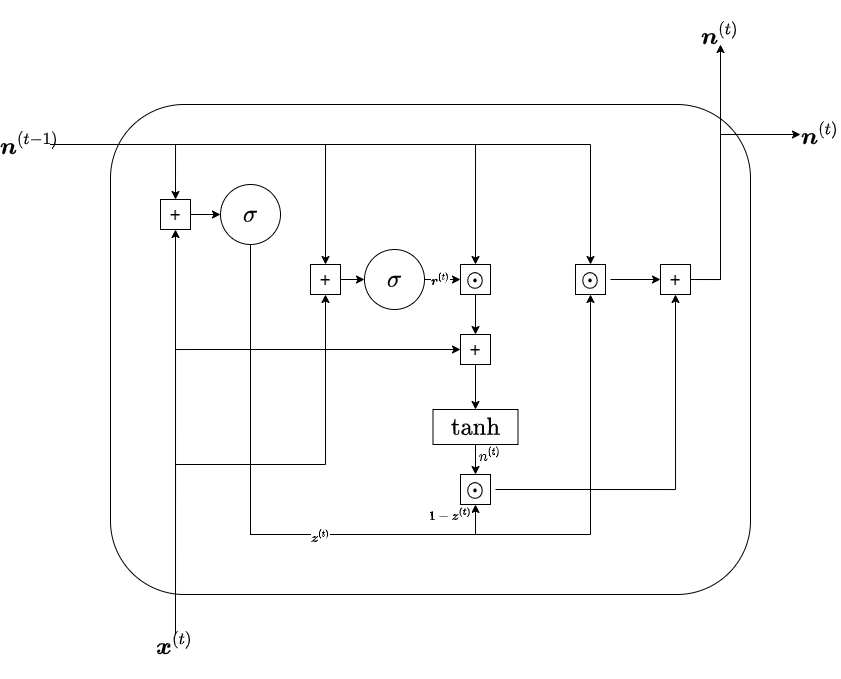
\includegraphics[width=\textwidth]{immagini/6_4/gruSchema.drawio.png}
        \caption{}
        \label{fig:strutturaGRU}
    \end{figure}
\end{document}